\documentclass{article}

\usepackage[T1]{fontenc}

\usepackage{polski}
\usepackage[utf8]{inputenc}
\usepackage[polish]{babel}
\let\lll\undefined
\usepackage{amssymb}
\usepackage{amsmath}
\usepackage{algorithm}
\usepackage{algpseudocode}
\usepackage{graphicx}
\usepackage{floatpag}
\usepackage{subcaption}



\title{Pracownia z analizy numerycznej \\ Sprawozdanie do zadania P3.06}
\author{Mikołaj Słupiński}
\date{Wrocław, dnia 12 stycznia 2017 r.}

\begin{document}
  \maketitle
  \section{Wstęp}
    \paragraph{}Przybliżanie wartości całki oznaczonej jest jednym z najważniejszych
    zadań analizy numerycznej. Nic więc dziwnego, że powstało wiele metod całkowania
    numerycznego. Wśród nich, szczególną popularnością cieszą się kwadratura Gaussa
    oraz Newtona-Cotesa. Nie mniej popularną metodą jest metoda Curtisa-Clenshawa
    interpolująca funkcję w $n+1$ punktach, ekstremach wielomianu Czebyszewa. Opisywana
    przeze mnie kwadratura działa na podobnej zasadzie.

  \section{Opis kwadratury}
    \paragraph{} Niech $I$ będzie całką postaci
      \begin{equation*}
        I = \int_{-1}^{1}f(x)dx\,.
      \end{equation*}

    Niech $n \ge 2$ będzie ustaloną liczba parzystą. Możemy wtedy określić $n+1$
    węzłów interpolacyjnych na przedziale $[-1,1]$ w miejscu punktów ekstremalnych
    wielomianu Czebyszewa $T_{n}(x)$ oraz punktavh brzegowych, wtedy

      \begin{equation*}
        u_k := \cos{\alpha_k},\quad
        \alpha_k := \frac{k\pi}{n},\quad
        k = 0, 1, ..., n \,.
      \end{equation*}

    Te punkty pozwalają nam dokonać interpolacji Czebyszewa drugiego rodzaju.
    Możemy przybliżyć funkcję $f(x)$ przez wielomian $J_{n}(x)$ jako

    \begin{equation*}
      f(x) \approx J_n(x) = \sum_{k = 0}^{n}''a_{k}T(x)\,.
    \end{equation*}

    Wielomiany Czebyszewa są ortogonalne w sensie dyskretnego iloczynu skalarnego
    w węzłach $u_k$, co więcej

    \begin{equation*}
      \sum_{k=0}^{n}T_r(u_k)T_s(u_k) =
        \begin{cases}
          n       & \quad \text{jeżeli } r = s = 0 \text{ lub } r = s = n\\
          \frac{n}{2}  & \quad \text{jeżeli } r = s \neq 0 \\
        \end{cases}\,.
    \end{equation*}

    Otrzymujemy w ostateczności

    \begin{equation*}
      a_k = \frac{2}{n} \sum_{j = 0}{n}'' f(u_j)T_k(u_j)\,.
    \end{equation*}

    Niech $J_n$ będzie naszym przybliżeniem funkcji $f$. Pozwala nam  ono aproksymować
    wartość całki $I$. Zdefiniujmy $I_n$ następująco:

    \begin{equation*}
      I_n := \int_{-1}^{1}J_{n}(x)dx\,.
    \end{equation*}

    Z wzoru rekurencyjnego na kolejne wielomiany Czebyszewa otrzymujemy
    \begin{equation*}
      \int_{-1}^{1}T_{n}(x)dx = \frac{1}{2}\Big(\frac{T_{n+1}(x)}{n+1} - \frac{T_{n-1}(x)}{n-1}\Big)\Big|_{-1}^1\,.
    \end{equation*}

    Korzystając z powyższego wzoru ostatecznie dostajemy

    \begin{equation*}
      I_n = 2(b_1 + b_3 + ... + b_{n-1}),\quad \text{gdzie } b_{2k-1} := \frac{a_{2k-2} - a_{2k}}{4k-2}\,.
    \end{equation*}

    Powyższy wzór pozwala nam na przybliżenie całki z satysfakcjonującą dokładnością.
  \section{Przykłady obliczeń}
    \paragraph{} Aby uzmysłowić sobie działanie powyższej metody, warto dokonać kilku przykładowych
    obliczeń. Do wykonania testów użyto programu \texttt{program.jl}.

    \begin{figure}
      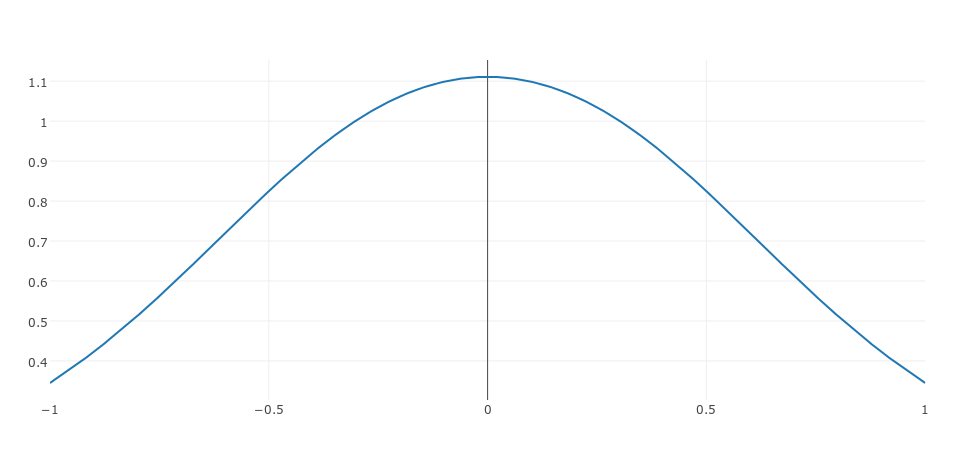
\includegraphics[width=\linewidth]{fplot.png}
      \caption{Wykres funkcji $f(x)$}
      \label{fig:fplot}
    \end{figure}

    Za pierwszy przykład posłuży nam funkcja $f(x)$ zdefiniowana następująco

    \begin{equation*}
      f(x) = \frac{1}{x^4 + x^2 + 0.9}\,,
    \end{equation*}
    dla której wartość całki wynosi

    \begin{equation*}
      \int_{-1}^{1} f(x)dx = 1.58223 \,.
    \end{equation*}

    W tabeli nr \ref{tab:f} pokazano wyniki przybliżeń wartości całki dla $n \in {2, 4, ..., 100}$.

    \begin{table}[htb]
      \centering
      \caption{Wartości kolejnych przybliżeń $I_n$ dla funkcji $f$}
      \label{tab:f}
      \begin{tabular}{|c|c|c|c|}
        \hline
        $n$ & $I_n$              & $n$ & $I_n$              \\ \hline
         2  & 1.8390804597701154 &  52 & 1.8390804597701154 \\
         4  & 1.5691396725879485 &  54 & 1.5691396725879485 \\
         6  & 1.5823077129642087 &  56 & 1.5823077129642087 \\
         8  & 1.5823677724538778 &  58 & 1.5823677724538778 \\
        10  & 1.5821874997277126 &  60 & 1.5821874997277126 \\
        12  & 1.5822408404681412 &  62 & 1.5822408404681412 \\
        14  & 1.5822322569562068 &  64 & 1.5822322569562068 \\
        16  & 1.5822329156419064 &  66 & 1.5822329156419064 \\
        18  & 1.5822329978953582 &  68 & 1.5822329978953582 \\
        20  & 1.5822329560919610 &  70 & 1.5822329560919610 \\
        22  & 1.5822329647058602 &  72 & 1.5822329647058602 \\
        24  & 1.5822329637106787 &  74 & 1.5822329637106787 \\
        26  & 1.5822329637029517 &  76 & 1.5822329637029517 \\
        28  & 1.5822329637376509 &  78 & 1.5822329637376509 \\
        30  & 1.5822329637283628 &  80 & 1.5822329637283628 \\
        32  & 1.5822329637297676 &  82 & 1.5822329637297676 \\
        34  & 1.5822329637296915 &  84 & 1.5822329637296915 \\
        36  & 1.5822329637296630 &  86 & 1.5822329637296630 \\
        38  & 1.5822329637296730 &  88 & 1.5822329637296730 \\
        40  & 1.5822329637296740 &  90 & 1.5822329637296740 \\
        42  & 1.5822329637296728 &  92 & 1.5822329637296728 \\
        44  & 1.5822329637296710 &  94 & 1.5822329637296710 \\
        46  & 1.5822329637296735 &  96 & 1.5822329637296735 \\
        48  & 1.5822329637296715 &  98 & 1.5822329637296715 \\
        50  & 1.5822329637296755 & 100 & 1.5822329637296755 \\ \hline
      \end{tabular}
    \end{table}

    \begin{figure}
      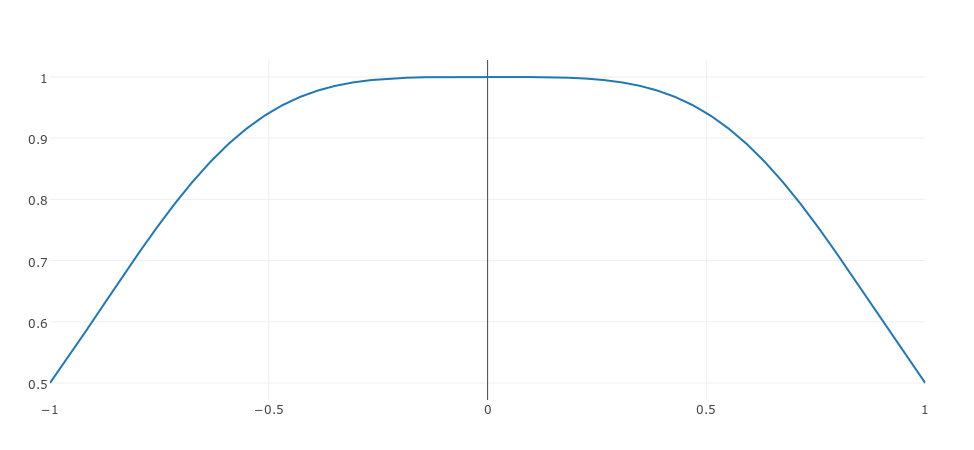
\includegraphics[width=\linewidth]{gplot.png}
      \caption{Wykres funkcji $g(x)$}
      \label{fig:gplot}
    \end{figure}

    Spróbujmy teraz rozważyć następującą funkcję
    \begin{equation*}
      g(x) = \frac{1}{1 + x^4}\,,
    \end{equation*}
    dla której wartość całki na przedziale $[0, 1]$ wynosi:

    \begin{equation*}
      \int_{0}^{1} g(x)dx = \frac{2\pi - \log(17 - 12\sqrt{2})}{8\sqrt{2}} \approx 0.86697\,.
    \end{equation*}

    Zauważmy, że funkcja $g(x)$ jest parzysta, a zatem możemy obliczyć jej wartość
    na przedziale $[-1, 1]$, a następnie wynik podzielić przez dwa. Wyniki kolejnych
    przybliżeń wartości funkcji $g$ podano w tabeli nr \ref{tab:g}.

    \begin{table}[htb]
      \centering
      \caption{Wartości kolejnych przybliżeń $I_n$ dla funkcji $g$}
      \label{tab:g}
      \begin{tabular}{|c|c|c|c|}
        \hline
        $n$ & $I_n$              & $n$ & $I_n$              \\ \hline
          2 & 0.8750000000000000 &  52 & 0.8750000000000000 \\
          4 & 0.8624999999999999 &  54 & 0.8624999999999999 \\
          6 & 0.8661764705882353 &  56 & 0.8661764705882353 \\
          8 & 0.8670717446270544 &  58 & 0.8670717446270544 \\
         10 & 0.8669927009342300 &  60 & 0.8669927009342300 \\
         12 & 0.8669664978194389 &  62 & 0.8669664978194389 \\
         14 & 0.8669732969416176 &  64 & 0.8669732969416176 \\
         16 & 0.8669731743756107 &  66 & 0.8669731743756107 \\
         18 & 0.8669729457800330 &  68 & 0.8669729457800330 \\
         20 & 0.8669729869401689 &  70 & 0.8669729869401689 \\
         22 & 0.8669729890232729 &  72 & 0.8669729890232729 \\
         24 & 0.8669729870778224 &  74 & 0.8669729870778224 \\
         26 & 0.8669729873159584 &  76 & 0.8669729873159584 \\
         28 & 0.8669729873545489 &  78 & 0.8669729873545489 \\
         30 & 0.8669729873384345 &  80 & 0.8669729873384345 \\
         32 & 0.8669729873395545 &  82 & 0.8669729873395545 \\
         34 & 0.8669729873400329 &  84 & 0.8669729873400329 \\
         36 & 0.8669729873399047 &  86 & 0.8669729873399047 \\
         38 & 0.8669729873399056 &  88 & 0.8669729873399056 \\
         40 & 0.8669729873399129 &  90 & 0.8669729873399129 \\
         42 & 0.8669729873399107 &  92 & 0.8669729873399107 \\
         44 & 0.8669729873399102 &  94 & 0.8669729873399102 \\
         46 & 0.8669729873399112 &  96 & 0.8669729873399112 \\
         48 & 0.8669729873399102 &  98 & 0.8669729873399102 \\
         50 & 0.8669729873399125 & 100 & 0.8669729873399125 \\ \hline
      \end{tabular}
    \end{table}

    \begin{figure}
      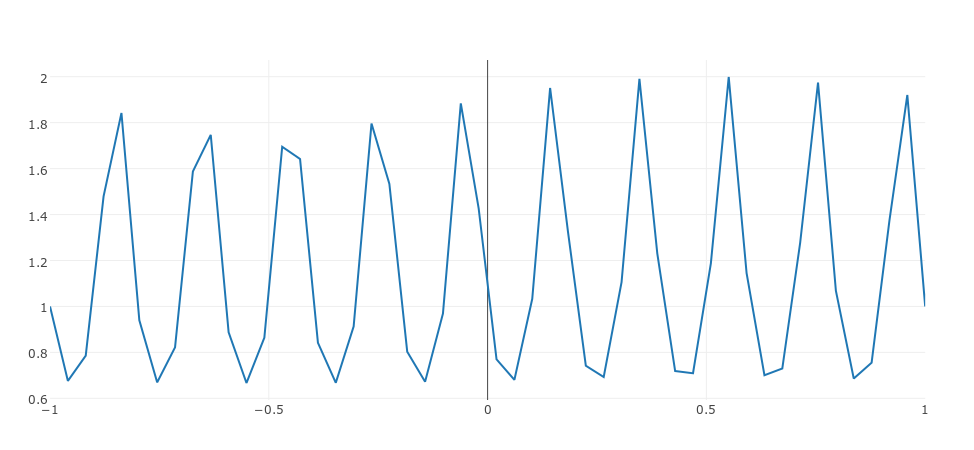
\includegraphics[width=\linewidth]{hplot.png}
      \caption{Wykres funkcji $h(x)$}
      \label{fig:hplot}
    \end{figure}

    Na samym końcu zdefiniujmy funkcję $h$ następująco:
    \begin{equation*}
      h(x) = \frac{2}{2 + \sin(10\pi x)}\,.
    \end{equation*}
    Wartość jej całki na przedziale $[-1, 1]$ wynosi

    \begin{equation*}
      \int_{-1}^{1} h(x)dx = \frac{4}{\sqrt{3}} \approx 2.3094 \,.
    \end{equation*}

    Kolejne przybliżenia przedstawiono w tabeli nr \ref{fig:hplot}.
    \begin{table}[htb]
      \centering
      \caption{Wartości kolejnych przybliżeń $I_n$ dla funkcji $h$}
      \label{tab:h}
      \begin{tabular}{|c|c|c|c|}
        \hline
        $n$ & $I_n$              & $n$ & $I_n$              \\ \hline
          2 & 1.9999999999999987 &  52 & 1.9999999999999987 \\
          4 & 2.0144763777856167 &  54 & 2.0144763777856167 \\
          6 & 2.1318513910770880 &  56 & 2.1318513910770880 \\
          8 & 2.1026132264713615 &  58 & 2.1026132264713615 \\
         10 & 2.1066815288634750 &  60 & 2.1066815288634750 \\
         12 & 2.2545974763952747 &  62 & 2.2545974763952747 \\
         14 & 2.2300844342456890 &  64 & 2.2300844342456890 \\
         16 & 2.2116395861568248 &  66 & 2.2116395861568248 \\
         18 & 2.3716382456932217 &  68 & 2.3716382456932217 \\
         20 & 2.2493862059556147 &  70 & 2.2493862059556147 \\
         22 & 2.3966957951946326 &  72 & 2.3966957951946326 \\
         24 & 2.2135598288329947 &  74 & 2.2135598288329947 \\
         26 & 2.4171205361186754 &  76 & 2.4171205361186754 \\
         28 & 2.2713032539077330 &  78 & 2.2713032539077330 \\
         30 & 2.1510751250836493 &  80 & 2.1510751250836493 \\
         32 & 2.2227420660882120 &  82 & 2.2227420660882120 \\
         34 & 2.2898488541296260 &  84 & 2.2898488541296260 \\
         36 & 2.3050764298124040 &  86 & 2.3050764298124040 \\
         38 & 2.3073904328059040 &  88 & 2.3073904328059040 \\
         40 & 2.3139707445860160 &  90 & 2.3139707445860160 \\
         42 & 2.3052286725846383 &  92 & 2.3052286725846383 \\
         44 & 2.3131874756999620 &  94 & 2.3131874756999620 \\
         46 & 2.3040080041515925 &  96 & 2.3040080041515925 \\
         48 & 2.3146045892301577 &  98 & 2.3146045892301577 \\
         50 & 2.3056929418149905 & 100 & 2.3056929418149905 \\ \hline
      \end{tabular}
    \end{table}

  \section{Dokładność zastosowanej kwadratury}
    \paragraph{} Stosując daną kwadraturę warto znać jej dokładność, żeby wiedzieć
    jak dobry wynik przybliżenia otrzymujemy. Jednakże, nie zawsze jesteśmy w stanie
    obliczyć błąd kolejnych przybliżeń.

    Rozwiązaniem problemu może okazać się eksperymentalne sprawdzenie, w jaki sposób
    różnią się między sobą kolejne przybliżenia funkcji, po to aby tak dobrać wartość
    $n$, aby przybliżenie było stosunkowo dokładne.

    Chcemy aby wartości przybliżeń spełniały nierówność

    \begin{equation*}
        |I_n - I_{n-2}| < \varepsilon |I_{n}|
    \end{equation*}
    dla ustalonego $\varepsilon$.

    W tabeli nr \ref{tab:errestimations} pokazano wartości wyrażenia
    $\frac{|I_n - I_{n-2}|}{|I_{n}|}$ dla kolejnych wartości $n$. Widać, że już dla
    $n$ równego około 40, jesteśmy w stanie uzyskać satysfakcjonujące nas przybliżenie.
  \begin{table}[htb]
    \centering
    \caption{Wartości kolejnych względnych zmian przybliżeń całki}
    \label{tab:errestimations}
    \begin{tabular}{|l|l|l|l|}
      \hline
      $n$ & $f(x)$                        & $g(x)$                        & $h(x)$                       \\ \hline
      4   & $0.1720310766$                & $0.0144927536$                & $0.0071861740$               \\
      6   & $0.0083220478$                & $0.0042444822$                & $0.0550577839$               \\
      8   & $3.7955455561 \cdot 10^{-5} $ & $0.0010325259$                & $0.0139056314$               \\
      10  & $0.0001139389$                & $9.1169963414 \cdot 10^{-5} $ & $0.0019311426$               \\
      12  & $3.3712149923 \cdot 10^{-5} $ & $3.0223906987 \cdot 10^{-5} $ & $0.0656063661$               \\
      14  & $5.4249380245 \cdot 10^{-6} $ & $7.8423663136 \cdot 10^{-6} $ & $0.0109919794$               \\
      16  & $4.1630135047 \cdot 10^{-7} $ & $1.4137231753 \cdot 10^{-7} $ & $0.0083398978$               \\
      18  & $5.1985675900 \cdot 10^{-8} $ & $2.6367094706 \cdot 10^{-7} $ & $0.0674633494$               \\
      20  & $2.6420507187 \cdot 10^{-8} $ & $4.7475684335 \cdot 10^{-8} $ & $0.0543490662$               \\
      22  & $5.4441408703 \cdot 10^{-9} $ & $2.4027323215 \cdot 10^{-9} $ & $0.0614636157$               \\
      24  & $6.2897279705 \cdot 10^{-10}$ & $2.2439574201 \cdot 10^{-9} $ & $0.0827336871$               \\
      26  & $4.8835603758 \cdot 10^{-12}$ & $2.7467517314 \cdot 10^{-10}$ & $0.0842162003$               \\
      28  & $2.1930482585 \cdot 10^{-11}$ & $4.4511726119 \cdot 10^{-11}$ & $0.0641998297$               \\
      30  & $5.8702643902 \cdot 10^{-12}$ & $1.8586890625 \cdot 10^{-11}$ & $0.0558921106$               \\
      32  & $8.8790731047 \cdot 10^{-13}$ & $1.2918430027 \cdot 10^{-12}$ & $0.0322425810$               \\
      34  & $4.8135325982 \cdot 10^{-14}$ & $5.5179931589 \cdot 10^{-13}$ & $0.0293062085$               \\
      36  & $1.7963037101 \cdot 10^{-14}$ & $1.4790629145 \cdot 10^{-13}$ & $0.0066061045$               \\
      38  & $6.3151302309 \cdot 10^{-15}$ & $1.0244591616 \cdot 10^{-15}$ & $0.0010028658$               \\
      40  & $5.6134490942 \cdot 10^{-16}$ & $8.4517880828 \cdot 10^{-15}$ & $0.0028437316$               \\
      42  & $7.0168113677 \cdot 10^{-16}$ & $2.5611479039 \cdot 10^{-15}$ & $0.0037922797$               \\
      44  & $1.1226898188 \cdot 10^{-15}$ & $5.1222958077 \cdot 10^{-16}$ & $0.0034406217$               \\
      46  & $1.5436985009 \cdot 10^{-15}$ & $1.1525165567 \cdot 10^{-15}$ & $0.0039841318$               \\
      48  & $1.2630260462 \cdot 10^{-15}$ & $1.1525165567 \cdot 10^{-15}$ & $0.0045781405$               \\
      50  & $2.5260520924 \cdot 10^{-15}$ & $2.5611479039 \cdot 10^{-15}$ & $0.0038650625$               \\
      52  & $1.6840347282 \cdot 10^{-15}$ & $2.1769757183 \cdot 10^{-15}$ & $0.0015727278$               \\
      54  & $1.8243709556 \cdot 10^{-15}$ & $1.4086313471 \cdot 10^{-15}$ & $0.0021533167$               \\
      56  & $8.4201736412 \cdot 10^{-16}$ & $2.5611479039 \cdot 10^{-16}$ & $0.0048830083$               \\
      58  & $1.4033622735 \cdot 10^{-15}$ & $1.4086313471 \cdot 10^{-15}$ & $0.0018468347$               \\
      60  & $1.8243709556 \cdot 10^{-15}$ & $1.5366887423 \cdot 10^{-15}$ & $0.0050319894$               \\
      62  & $2.5260520924 \cdot 10^{-15}$ & $2.3050331135 \cdot 10^{-15}$ & $0.0006724679$               \\
      64  & $1.8243709556 \cdot 10^{-15}$ & $2.0489183231 \cdot 10^{-15}$ & $0.0015999044$               \\
      66  & $2.5260520924 \cdot 10^{-15}$ & $3.4575496702 \cdot 10^{-15}$ & $0.0013339440$               \\
      68  & $1.9647071830 \cdot 10^{-15}$ & $2.3050331135 \cdot 10^{-15}$ & $0.0004871373$               \\
      70  & $4.7714317300 \cdot 10^{-15}$ & $5.6345253885 \cdot 10^{-15}$ & $3.3208326070 \cdot 10^{-5}$ \\
      72  & $1.9647071830 \cdot 10^{-15}$ & $1.4086313471 \cdot 10^{-15}$ & $0.0001529252$               \\
      74  & $9.8235359148 \cdot 10^{-16}$ & $7.6834437117 \cdot 10^{-16}$ & $0.0001050872$               \\
      76  & $1.4033622735 \cdot 10^{-15}$ & $2.3050331135 \cdot 10^{-15}$ & $1.1012104827 \cdot 10^{-5}$ \\
      78  & $4.0697505933 \cdot 10^{-15}$ & $5.1222958078 \cdot 10^{-15}$ & $0.0001845652$               \\
      80  & $4.7714317300 \cdot 10^{-15}$ & $5.1222958078 \cdot 10^{-15}$ & $0.0002735047$               \\
      82  & $9.8235359148 \cdot 10^{-16}$ & $1.1525165567 \cdot 10^{-15}$ & $0.0001803354$               \\
      84  & $1.4033622735 \cdot 10^{-16}$ & $5.1222958078 \cdot 10^{-16}$ & $8.6652674217 \cdot 10^{-5}$ \\
      86  & $4.2100868206 \cdot 10^{-16}$ & $2.5611479039 \cdot 10^{-16}$ & $0.0002736495$               \\
      88  & $8.4201736412 \cdot 10^{-16}$ & $7.6834437117 \cdot 10^{-16}$ & $2.2295008466 \cdot 10^{-5}$ \\
      90  & $1.5436985008 \cdot 10^{-15}$ & $2.1769757183 \cdot 10^{-15}$ & $0.0002757381$               \\
      92  & $0.0$                         & $0.0$                         & $0.0001034812$               \\
      94  & $4.9117679574 \cdot 10^{-15}$ & $6.7870419453 \cdot 10^{-15}$ & $5.5386735009 \cdot 10^{-5}$ \\
      96  & $3.6487419112 \cdot 10^{-15}$ & $5.3784105982 \cdot 10^{-15}$ & $0.0001008388$               \\
      98  & $2.3857158650 \cdot 10^{-15}$ & $3.4575496702 \cdot 10^{-15}$ & $7.6890799797 \cdot 10^{-5}$ \\
      100 & $7.0168113677 \cdot 10^{-16}$ & $0.0$                         & $1.4268564785 \cdot 10^{-5}$ \\ \hline

    \end{tabular}
  \end{table}

  \section{Wnioski}

    \paragraph{} Istnieje wiele różnych kwadratur pozwalających nam przybliżyć
    wartość całki. Jednakże, znając podstawowe zasady ich działania, jesteśmy w stanie
    modyfikować je oraz tworzyć własne. Dobrą bazą jest interpolacja wielomianowa
    funkcji, która jest podstawą m.in. kwadratury Newtona-Cotesa czy Curtisa-Clenshawa.

    Ponadto, zazwyczaj jesteśmy w stanie zoptymalizować powstałe kwadratury, np.
    w przypadku omówionej przez nas metody, możemy wykorzystać szybką transformatę
    Fouriera do obliczenia kolejnych współczynników naszego wielomianu interpolacyjnego.

    Nie zawsze jednak łatwo jest oszacować otrzymaną dokładność przybliżenia, ale mimo to
    jesteśmy w stanie dobrać parametry, aby dobrze ocenić uzyskane przybliżenie.

    \begin{thebibliography}{9}
      \bibitem{kincaid}
        David Kincaid, Ward Cheney,
        \textit{Analiza Numeryczna},
        Wydawnictwa Naukowo-Techniczne, Warszawa, 2006.

      \bibitem{bjorck}
        Ake Bj\"orck, Germund Dahlquist,
        \textit{Metody numeryczne},
        Państwowe Wydawnictwo Naukowe, 1987.

      \bibitem{jorg}
        J\"org Waldvogel
        \textit{Fast Construction of the Fej\'er and Clenshaw-Curtis Quadrature Rules},
        BIT Numerical Mathematics, 2003, Vol. 43, No. 1, pp. 001{018.
    \end{thebibliography}


\end{document}
